%auto-ignore



\section{BERT}
\label{sec:bert}

% BERT: what is pretraining and what is fine tuning at high level
We introduce BERT and its detailed implementation in this section. There are two steps in our framework: {\em pre-training} and {\em fine-tuning}. 
During pre-training, the model is trained on unlabeled data over different pre-training tasks.
For fine-tuning, the BERT model is first initialized with the pre-trained parameters, and all of the parameters are fine-tuned using labeled data from the downstream tasks. 
Each downstream task has separate fine-tuned models, even though they
are initialized with the same pre-trained parameters. The question-answering example in Figure~\ref{fig:bert_overall} will serve as a running example for this section.

A distinctive feature of BERT is its unified architecture across different tasks.
There is minimal difference between the pre-trained architecture and the final downstream architecture.

\paragraph{Model Architecture}
BERT's model architecture is a multi-layer bidirectional Transformer encoder based on the original implementation described in \citet{vaswani-etal:2017:_atten} and released in the {\tt tensor2tensor} library.\footnote{https://github.com/tensorflow/tensor2tensor} Because the use of Transformers has become common and our implementation is almost identical to the original, we will omit an exhaustive background description of the model architecture and refer readers to \citet{vaswani-etal:2017:_atten} as well as excellent guides such as ``The Annotated Transformer.''\footnote{http://nlp.seas.harvard.edu/2018/04/03/attention.html}

In this work, we denote the number of layers (i.e., Transformer blocks) as $L$, the hidden size as $H$, and the number of self-attention heads as $A$.\footnote{In all cases we set the feed-forward/filter size to be $4H$, i.e., 3072 for the $H=768$ and 4096 for the $H=1024$.} We primarily report results on two model sizes: {\bf \bertbase} (L=12, H=768, A=12, Total Parameters=110M) and {\bf \bertlarge} (L=24, H=1024, A=16, Total Parameters=340M).

\bertbase was chosen to have the same model size as OpenAI GPT for comparison purposes. Critically, however, the BERT Transformer uses bidirectional self-attention, while the GPT Transformer uses constrained self-attention where every token can only attend to context to its left.\footnote{We note that in the literature the bidirectional Transformer is often referred to as a ``Transformer encoder'' while the left-context-only version is referred to as a ``Transformer decoder'' since it can be used for text generation.} 


\paragraph{Input/Output Representations} % Claim we shared the structures
To make BERT handle a variety of down-stream tasks,
our input representation is able to unambiguously represent both a single sentence and a pair of  sentences (e.g., $\langle$ Question, Answer $\rangle$) in one token sequence. Throughout this work, a ``sentence'' can be an arbitrary span of contiguous text, rather than an actual linguistic sentence. A ``sequence'' refers to the input token sequence to BERT, which may be a single sentence or two sentences packed together.

We use WordPiece embeddings \cite{wu-etal:2016:_googl} with a 30,000 token vocabulary.
%We denote split word pieces with {\tt \#\#}. We use learned positional embeddings with supported sequence lengths up to 512 tokens.
The first token of every sequence is always a special classification token ({\tt [CLS]}). The final hidden state corresponding to this token is used as the aggregate sequence representation for classification tasks. 
%For non-classification tasks, this vector is ignored.
Sentence pairs are packed together into a single sequence. We differentiate the sentences in two ways. First, we separate them with a special token ({\tt [SEP]}). Second, we add a learned embedding to every token indicating whether it belongs to sentence {\tt A} or sentence {\tt B}. 
As shown in Figure~\ref{fig:bert_overall}, we denote 
input embedding as $E$, the final hidden vector of the special {\tt [CLS]} token as $C \in \mathbb{R}^{H}$, and the final hidden vector for the $i^{\rm th}$ input token as $T_i \in \mathbb{R}^H$.

For a given token, its input representation is constructed by summing the corresponding token, segment, and position embeddings. 
A visualization of this construction can be seen in Figure~\ref{fig:input_embeddings}.

\begin{figure*}[ht]
\begin{center}
\hspace{-0.2in}
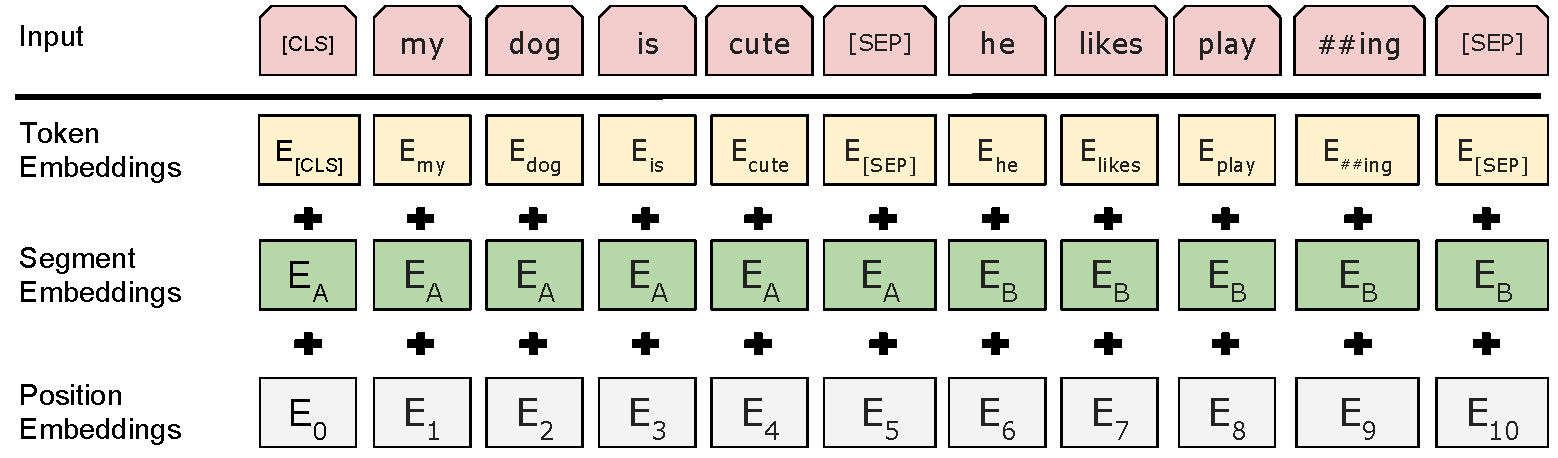
\includegraphics[width=360px]{Input_Emebeddings.pdf}
\end{center}
\caption{BERT input representation. The input embeddings are the sum of the token embeddings, the segmentation embeddings and the position embeddings.}
\label{fig:input_embeddings}
\end{figure*}


%In the subsequent model descriptions, 


\subsection{Pre-training BERT}
\label{sec:pretraining_tasks}

Unlike \citet{peters-etal:2018:_deep} and \citet{radford-etal:2018}, we do not use traditional left-to-right or right-to-left language models to pre-train BERT. Instead, we pre-train BERT using two unsupervised tasks, described in this section. This step
is presented in the left part of Figure~\ref{fig:bert_overall}.

%\noindent\textbf{Task \#1: Masked LM}
\paragraph{Task \#1: Masked LM}
Intuitively, it is reasonable to believe that a deep bidirectional model is strictly more powerful than either a left-to-right model or the shallow concatenation of a left-to-right and a right-to-left model. Unfortunately, standard conditional language models can only be trained left-to-right {\it or} right-to-left, since bidirectional conditioning would 
allow each word to indirectly ``see itself'', and
the model could trivially predict the target word in a multi-layered context.

In order to train a deep bidirectional representation, we simply mask some percentage of the input tokens at random, and then predict those masked tokens. We refer to this procedure as a ``masked LM'' (MLM), although it is often referred to as a {\it Cloze} task in the literature~\cite{taylor:1953:_cloze}. In this case, the final hidden vectors corresponding to the mask tokens are fed into an output softmax over the vocabulary, as in a standard LM. In all of our experiments, we mask 15\% of all WordPiece tokens in each sequence at random. In contrast to denoising auto-encoders \cite{vincent:2008}, we only predict the masked words rather than reconstructing the entire input.  
%Unlike \citet{melamud2016context2vec}, we mask multiple input tokens at the same time and train a deep bi-directional encoder instead of a top-level combination of left and right context encoders. In addition, we use additional token-level objectives more similar to ones in denoising auto-encoders and auto-encoders (see last two prediction tasks in the list below).

Although this allows us to obtain a bidirectional pre-trained model, a downside is that we are creating a mismatch between pre-training and fine-tuning, since the {\tt [MASK]} token does not appear during fine-tuning. To mitigate this, we do not always replace ``masked'' words with the actual {\tt [MASK]} token. The training data generator chooses 15\% of the token positions at random for prediction. If the $i$-th token is chosen, we replace the $i$-th token with (1) the {\tt [MASK]} token 80\% of the time (2) a random token 10\% of the time (3) the unchanged $i$-th token 10\% of the time. Then, $T_i$ will be used to predict the original token with cross entropy loss.
We compare variations of this procedure in Appendix~\ref{appendix:sec:different_masks}.
\vspace{.2cm}

%\noindent\textbf{Task \#2: Next Sentence Prediction (NSP)}
\paragraph{Task \#2: Next Sentence Prediction (NSP)}
Many important downstream tasks such as Question Answering (QA) and Natural Language Inference (NLI) are based on understanding the {\it relationship} between two sentences, which is not directly captured by language modeling. In order to train a model that understands sentence relationships, we pre-train for a binarized {\it next sentence prediction} task that can be trivially generated from any monolingual corpus. Specifically, when choosing the sentences {\tt A} and {\tt B} for each pre-training example, 50\% of the time {\tt B} is the actual next sentence that follows {\tt A} (labeled
 as {\tt {\small IsNext}}), and 50\% of the time it is a random sentence from the corpus
 (labeled as {\tt {\small NotNext}}). 
 %We choose the {\tt {\small NotNext}} sentences completely at random. 
As we show in Figure~\ref{fig:bert_overall}, $C$ is used for  next sentence prediction (NSP).\footnote{The final model achieves 97\%-98\% accuracy on NSP.} Despite its simplicity, we demonstrate in Section~\ref{sec:task_ablation} that pre-training towards this task is very beneficial to both QA and NLI.
\footnote{The vector $C$ is not a meaningful sentence representation without fine-tuning, since it was trained with NSP.}
The NSP task is closely related to representation-learning objectives used in \citet{DBLP:journals/corr/JerniteBS17} and \citet{logeswaran2018an}. However, in prior work, only sentence embeddings are transferred to down-stream tasks, where BERT transfers all parameters to initialize end-task model parameters.



\vspace{.3cm}
\noindent\textbf{Pre-training data}
The pre-training procedure largely follows the existing literature on language model pre-training. For the pre-training corpus we use the BooksCorpus (800M words)~\cite{zhu:2015} and English Wikipedia (2,500M words). For Wikipedia we extract only the text passages and ignore lists, tables, and headers. It is critical to use a document-level corpus rather than a shuffled sentence-level corpus such as the Billion Word Benchmark \cite{chelba-etal:2013:_one} in order to extract long contiguous sequences.

\subsection{Fine-tuning BERT}
\label{sec:finetuning_procedure}

Fine-tuning is straightforward since the self-attention mechanism in the Transformer allows BERT to model many downstream tasks---whether they involve single text or text pairs---by swapping out the appropriate inputs and outputs.
For applications involving text pairs, a common pattern is to independently encode text pairs before applying bidirectional cross attention, such as~\newcite{parikh-etal:2016, bidaf}. BERT instead uses the self-attention mechanism to unify these two stages, as encoding 
a concatenated text pair with self-attention effectively includes \emph{bidirectional} cross attention between two sentences. 


For each task, we simply plug in the task-specific inputs and outputs into BERT and fine-tune all the parameters end-to-end. 
%
At the input, sentence {\tt A} and sentence {\tt B} from pre-training are analogous to (1) sentence pairs in paraphrasing, (2) hypothesis-premise pairs in entailment, (3) question-passage pairs in question answering, and (4) a degenerate text-$\varnothing$ pair in text classification or sequence tagging. At the output, the token representations are fed into an output layer for token-level tasks, such as sequence tagging or question answering, and the {\tt [CLS]} representation is fed into an output layer for classification, such as entailment or sentiment analysis.


Compared to pre-training, fine-tuning is relatively inexpensive. All of the results in the paper can be replicated in at most 1 hour on a single Cloud TPU, or a few hours on a GPU, starting from the exact same pre-trained model.\footnote{For example, the BERT SQuAD model can be trained in around 30 minutes on a single Cloud TPU to achieve a Dev F1 score of 91.0\%.}
We describe the task-specific details in the corresponding subsections of Section~\ref{sec:experiments}. 
More details can be found in Appendix~\ref{appendix:sec:fine_tune_details_and_figures}.


\eat{The standard pattern in many NLP models is to independently encode text pairs before apply bidirectional cross attention, such as ~\newcite{parikh-etal:2016, bidaf}. BERT instead leverages the self-attention mechanism in the Transformer to unify these two stages. Encoding with self-attention is performed jointly with \emph{iterative} and \emph{bidirectional} cross attention.
Therefore, many downstream tasks---whether they involve single text or text pairs---can be modeled by simply swapping out the appropriate inputs and outputs.

At the input, sentence {\tt A} and sentence {\tt B} from pre-training are analogous to (1) sentence pairs in paraphrasing, (2) hypothesis-premise pairs in entailment, (3) question-passage pairs in question answering, and (4) a degenerate text-$\varnothing$ pair in text classification or sequence tagging. At the output, the token representations are fed into an output layer for token-level tasks, such as sequence tagging or question answering, and the {\tt [CLS]} representation is fed into an output layer for classification, such as entailment or sentiment analysis.

During the fine-tuning stage, we simply plug in the task-specific inputs and outputs into BERT and fine-tune all the parameters end-to-end. We describe the task-specific details in the corresponding subsections of Section~\ref{sec:experiments}. In-depth task specific design figures are also shown in Appendix~\ref{appendix:sec:fine_tune_details_and_figures}.
}

\eat{
\vspace{.3cm}
\noindent\textbf{Cross-attention}
BERT is designed such that it does not distinguish between self-attention used within a single sequence and cross-attention used between multiple sequences. Cross-attention between
question and passage has been shown to be important for question-answering~\cite{bidaf}, where they cross
attend question and passage for two times.
When fine-tuning a twelve-layer BERT for question answering, the question and passage will cross attend to each other for {\em twelve} times given that question and passage are packed into a single input sequence
\emph{iteratively}. Moreover, the parameters for cross-attention are pretrained. The iterative attention also happened in OpenAI GPT, but
the second sequence cannot attend to the first sequence due to the unidirectionality constraint.
}